% ===========================================
% Template for ICMC 2021 in Santiago, Chile (version1)
% adapted from earlier LaTeX paper templates for the ICMC, SMC, etc...
% by Rodrigo F. Cádiz rcadiz@uc.cl
% ===========================================

\documentclass{article}
\usepackage{icmc2021template}
\usepackage{times}
\usepackage{ifpdf}
\usepackage{soul}
\usepackage[english]{babel}
\usepackage{enumitem}
\usepackage{musicography}
\usepackage{amsmath}
\usepackage{arydshln}
\usepackage{amssymb}
\usepackage{caption}
\captionsetup{skip=5pt}
\usepackage{graphics}
 \usepackage{musicography}
%\usepackage{cite}


\usepackage{calc}
\newlength{\maxcollen}

\newcommand{\setmeter}[2]{\ensuremath{%
  \vcenter{\offinterlineskip
    \halign{\hfil##\hfil\cr
            $\scriptstyle#1$\cr
            \noalign{\vskip1pt}
            $\scriptstyle#2$\cr}
  }}%
}

%%%%%%%%%%%%%%%%%%%%%%%% Some useful packages %%%%%%%%%%%%%%%%%%%%%%%%%%%%%%%
%%%%%%%%%%%%%%%%%%%%%%%% See related documentation %%%%%%%%%%%%%%%%%%%%%%%%%%
%\usepackage{amsmath} % popular packages from Am. Math. Soc. Please use the 
%\usepackage{amssymb} % related math environments (split, subequation, cases,
%\usepackage{amsfonts}% multline, etc.)
%\usepackage{bm}      % Bold Math package, defines the command \bf{}
%\usepackage{paralist}% extended list environments
%%subfig.sty is the modern replacement for subfigure.sty. However, subfig.sty 
%%requires and automatically loads caption.sty which overrides class handling 
%%of captions. To prevent this problem, preload caption.sty with caption=false 
%\usepackage[caption=false]{caption}
%\usepackage[font=footnotesize]{subfig}

% ====================================================
% ================ Define title and author names here ===============
% ====================================================
%user defined variables
\def\papertitle{MusAssist: A Domain Specific Language for Music Notation}
\def\firstauthor{Ilana Shapiro}

% adds the automatic
% Saves a lot of output space in PDF... after conversion with the distiller
% Delete if you cannot get PS fonts working on your system.

% pdf-tex settings: detect automatically if run by latex or pdflatex
\newif\ifpdf
\ifx\pdfoutput\relax
\else
   \ifcase\pdfoutput
      \pdffalse
   \else
      \pdftrue
  \fi
\fi

\ifpdf % compiling with pdflatex
  \usepackage[pdftex,
    pdftitle={\papertitle},
    pdfauthor={\firstauthor},
    bookmarksnumbered, % use section numbers with bookmarks
    pdfstartview=XYZ % start with zoom=100% instead of full screen; 
                     % especially useful if working with a big screen :-)
   ]{hyperref}
  %\pdfcompresslevel=9

  \usepackage[pdftex]{graphicx}
  % declare the path(s) where your graphic files are and their extensions so 
  %you won't have to specify these with every instance of \includegraphics
  \graphicspath{{./figures/}}
  \DeclareGraphicsExtensions{.pdf,.jpeg,.png}

  \usepackage[figure,table]{hypcap}

\else % compiling with latex
  \usepackage[dvips,
    bookmarksnumbered, % use section numbers with bookmarks
    pdfstartview=XYZ % start with zoom=100% instead of full screen
  ]{hyperref}  % hyperrefs are active in the pdf file after conversion

  \usepackage[dvips]{epsfig,graphicx}
  % declare the path(s) where your graphic files are and their extensions so 
  %you won't have to specify these with every instance of \includegraphics
  \graphicspath{{./figures/}}
  \DeclareGraphicsExtensions{.eps}

  \usepackage[figure,table]{hypcap}
\fi

%setup the hyperref package - make the links black without a surrounding frame
\hypersetup{
    colorlinks,%
    citecolor=black,%
    filecolor=black,%
    linkcolor=black,%
    urlcolor=black
}


% ====================================================
% ================ Title and author info starts here ===============
% ====================================================
% Title.
% ------
\title{\papertitle}

% Authors
% Please note that submissions are anonymous, therefore 
% authors' names should not be VISIBLE in your paper submission.
% They should only be included in the camera-ready version of accepted papers.
% uncomment and use the appropriate section (1, 2 or 3 authors)
%
% Single address
% To use with only one author or several with the same address
% ---------------
%\oneauthor
%   {\firstauthor} {Affiliation \\ %
%     {\tt \href{mailto:author@uc.cl}{author@uc.cl}}}

%Two addresses
% the default spacing is 1.5in, but this can be reduced to 0.5in or less, if needed
%--------------
% \twoauthors
%   {1.5in}
%   {\firstauthor} {Affiliation1 \\  %
%     {\tt \href{mailto:author1@uc.cl}{author1@uc.cl}}}
%   {\secondauthor} {Affiliation2 \\  %
%     {\tt \href{mailto:author2@uc.cl}{author2@uc.cl}}}

% Three addresses
% the default spacing is 0.5in, but this can be reduced to 0.3in or less, if needed
% --------------
 \oneauthor
  %  {0.5in}
   {\firstauthor} {Pomona College \\ %
     {\tt \href{mailto:issa2018@mymail.pomona.edu}{issa2018@mymail.pomona.edu}}}
  %  {\secondauthor} {Affiliation2 \\ %
  %    {\tt \href{mailto:author2@myorg.org}{author2@myorg.org}}}
  %  {\thirdauthor} { Affiliation3 \\ %
  %    {\tt \href{mailto:author3@myorg.org}{author3@myorg.org}}}

% Four addresses
% the default spacing is 1.5in, but this can be reduced to 0.5in or less, if needed
% --------------
% \fourauthors
%   {1.5in}
%   {\firstauthor} {Affiliation1 \\ %
%     {\tt \href{mailto:author1@uc.cl}{author1@uc.cl}}}
%   {\secondauthor} {Affiliation2 \\ %
%     {\tt \href{mailto:author2@uc.cl}{author2@uc.cl}}}
%   {\thirdauthor} { Affiliation3 \\ %
%     {\tt \href{mailto:author3@uc.cl}{author3@uc.cl}}}
%   {\fourthauthor} { Affiliation4 \\ %
%     {\tt \href{mailto:author4@uc.cl}{author4@uc.cl}}}

% Five addresses
% the default spacing is 0.5in, but this can be reduced to 0.3in or less, if needed
% --------------
% \fiveauthors
%   {0.5in}
%   {\firstauthor} {Affiliation1 \\ %
%     {\tt \href{mailto:author1@uc.cl}{author1@uc.cl}}}
%   {\secondauthor} {Affiliation2 \\ %
%     {\tt \href{mailto:author2@uc.cl}{author2@uc.cl}}}
%   {\thirdauthor} { Affiliation3 \\ %
%     {\tt \href{mailto:author3@uc.cl}{author3@uc.cl}}}
%   {\fourthauthor} { Affiliation4 \\ %
%     {\tt \href{mailto:author4@uc.cl}{author4@uc.cl}}}
%   {\fifthauthor} { Affiliation5 \\ %
%     {\tt \href{mailto:author5@uc.cl}{author5@uc.cl}}}

% Six addresses
% the default spacing is 0.5in, but this can be reduced to 0.3in or less, if needed
% --------------
% \sixauthors
%   {0.5in}
%   {\firstauthor} {Affiliation1 \\ %
%     {\tt \href{mailto:author1@uc.cl}{author1@uc.cl}}}
%   {\secondauthor} {Affiliation2 \\ %
%     {\tt \href{mailto:author2@uc.cl}{author2@uc.cl}}}
%   {\thirdauthor} { Affiliation3 \\ %
%     {\tt \href{mailto:author3@uc.cl}{author3@uc.cl}}}
%   {\fourthauthor} { Affiliation4 \\ %
%     {\tt \href{mailto:author4@uc.cl}{author4@uc.cl}}}
%   {\fifthauthor} { Affiliation5 \\ %
%     {\tt \href{mailto:author5@uc.cl}{author5@uc.cl}}}
%   {\sixthauthor} { Affiliation6 \\ %
%     {\tt \href{mailto:author6@uc.cl}{author6@uc.cl}}}


% ====================================================
% =============== The document content starts here ===============
% ====================================================
\begin{document}
%
\capstartfalse
\maketitle
\capstarttrue
%
\begin{abstract}
MusAssist is an external, declarative, domain specific language for music notation that bridges the abstraction gap between music theory and composition. Users can describe high-level templates for chords and arpeggios (all triads and seventh chords), scales (diatonic, chromatic and whole tone), the five primary cadences, and the four primary harmonic sequences with desired length. Uniquely, MusAssist matches the level of abstraction of a template to the theoretical musical structure it describes (e.g. users can specify a harmonic sequence without needing to manually expand it to the chords and notes it comprises). Thus, users can write out specifications precisely at the conceptual levels of the musical structures they would organically conceive when composing by hand. In MusAssist, users can also change key signatures, start a new measure, and describe fundamental musical objects such as notes, rests, and customized chords. The Haskell-based MusAssist compiler expands high-level templates (thus lowering the level of abstraction to individual notes) and translates the program to MusicXML, a language accepted by most major music notation software, for further manual editing and playback.
\end{abstract}


\section{Introduction}\label{sec:introduction}
When writing music, composers must manually transition from theoretical musical concepts to notes on a page. This process can be tedious and slow, requiring the composer to expand complex musical structures by hand, such as cadences and harmonic sequences, to the individual notes they define. Therefore, the level of abstraction of the musical structure is higher than what the composer writes.

Domain specific languages (DSLs) are programming languages highly specialized for a specific application and thus characterized by limited expressiveness. An \textit{external} DSL has custom syntax that is separated from the primary language of its application.

This paper presents MusAssist, an external, declarative DSL for music notation that bridges the abstraction divide between music theory and notation. Users describe a composition in MusAssist’s straightforward, high-level syntax, modeled around the musical elements composers organically conceive when writing by hand, and the MusAssist compiler automates the expansion of these elements to their
constituent notes. MusAssist’s declarative programming paradigm was chosen to correspond with the lack of control structures in handwritten music.

MusAssist is unique in that users can encode specifications for complex musical templates at the same level of abstraction as the theoretical musical structures they describe. Specifically,  users can specify high-level templates for 
\textbf{chords} and \textbf{arpeggios} (major, minor, dominant, augmented, half diminished, and diminished triads and seventh chords in any inversion), 
\textbf{scales} (major, natural/harmonic/ melodic minor, chromatic, and whole tone), 
\textbf{cadences} (perfect authentic, imperfect authentic, plagal, half, deceptive), and 
\textbf{harmonic sequences} (ascending fifths, descending fifths, ascending 5-6, descending 5-6) of a desired length. MusAssist also supports individual notes, rests, and customized chords consisting of user-defined collections of notes, and enables the user to change the key signature or start a new measure. All high-level templates are expanded, lowering the abstraction level to notes, by the Haskell-based MusAssist compiler.

The target language of the MusAssist compiler is MusicXML, itself a DSL that is an extension of XML (Extensible Markup Language). MusicXML is accepted by most major notation software, such as MuseScore. Thus, users can open the resulting MusicXML file of a compiled MusAssist composition in MuseScore or another program for further customization and editing. Beyond a professional music compositional aid, MusAssist may be particularly helpful to music theory students as an educational tool, enabling them to visualize the relationship between a theoretical musical structure and its expanded form, such as in understanding the chords resulting from the expansion of a cadence. 

This paper first summarizes related work in music notation DSLs. Then, features of the MusAssist language are outlined, followed by the presentation of a practical use case. Finally, the structure of the MusAssist compiler and the central logic behind its automated template expansions are described. 


%-----------------------------------------------------------------------------------------------------------------------------------------------------

\section{Related Work}\label{sec:related_work}

The era of music DSLs began in 2008 with Ge Wang’s ChucK audio processing language for sound synthesis. With ChucK, Wang introduced the notion of ``strongly-timed” programming, in which users control the flow of time in their programs to arbitrarily fine granularities. ChucK also supports ``on-the-fly” programming, often referred to as live coding, where users can modify programs while they run. Together, these features allow ChucK to accurately and expressively simulate music performance and creation \cite{wang_2008}. 

Since then, computer scientists have taken advantage of the increased flexibility afforded to DSLs via their limited expressiveness to create music DSLs tailored towards notation, algorithmic composition, signal processing, live coding with music performance, and more. Aside from MusAssist, MusicXML, LilyPond, and PyTabs are commonly used music DSLs also specializing in notation.

Michael Good’s MusicXML is an Internet-friendly, XML-based, declarative DSL that represents standard Western music notation and scoring practices. Similar to how the popular MIDI format helped create a standardized format for electronic instruments, MusicXML provides a standardized format for online sheet music in order to create a standardized method for representing complex, structured musical data to support smooth interchange between musical applications specializing in notation, performance, analysis, music information retrieval, and more.\cite{good_2013}

To achieve this, Good derives MusicXML from XML due to its Internet-friendly nature, straightforward use in document creation, and human readability. In contrast, MIDI is very difficult to read and write, and is also less powerful and expressive than XML  \cite{good_2001}

MusicXML is more expressive than MusAssist, but the abstraction level of all musical elements is extremely low (i.e. chords must be written out as individual notes) and though easily readable, its syntax is cumbersome and tedious to write by hand. However, its enhanced expressiveness makes MusicXML an excellent target compilation language for MusAssist’s user-friendly syntax and high-level theoretical musical templates.

LilyPond, an external declarative DSL created by Han-Wen Nienhuys and Jan Nieuwenhuizen, is similar to MusAssist. It features a “modular, extensible and programmable compiler” written in Scheme to generate Western music notation of excellent quality, and supports the mixing of text and music elements. Text-based musical expressions, or fragments of music with set durations, are compiled to an aesthetically formatted score \cite{nienhuys_nieuwenhuizen_2003}

LilyPond and MusAssist are both music notation DSLs tailored to non-programming audiences. However, they differ in two fundamental areas: (1) MusAssist supports complex music templates at the levels of abstraction of the musical structures they represent, whereas LilyPond only supports granular, low level composition of individual notes and chords, and (2) the output of the MusAssist compiler is intentionally editable via notation software, unlike LilyPond’s compiler, which produces a static, printable PostScript or PDF file by taking in a file with a formal representation of the desired music. 
\cite{nienhuys_nieuwenhuizen_2003}

Simic et al.’s external, declarative DSL PyTabs similarly is geared toward music notation, but in a different domain than MusAssist. Specifically, the authors attempt to solve visual problem of tablature notation and the lack of standardization of how to specify note duration in this format by consolidating these issues into a formal language. Tablature notation is outside the scope of MusAssist’s focus on Western musical theoretical structures. 
 \cite{simic_bal_dejanovic_vaderna}.

%-----------------------------------------------------------------------------------------------------------------------------------------------------

\section{Language Features}\label{sec:language_features}
\subsection{Low-Level Fundamentals}
On the most basic level, MusAssist supports individual rests and notes. Rests are given a duration from sixteenth to whole note, and notes are further defined by note name (A to G), accidental (double flat to double sharp), and octave (1 to 8, after the range of a piano). Just as in normal notation, the absence of an accidental indicates natural quality. Users can also define customized chords, or user-defined lists of individual notes. These are not considered templates as the high-level description of the chord is not given, and the granularity is at the note level.

\subsection{High-Level Templates}
MusAssist supports templates for chords, arpeggios, scales, cadences, and harmonic sequences, specified uniquely at the abstraction level of the theoretical musical structures they represent.

Following the principles of music theory, chords are specified by their root note, quality (major, minor, augmented, dominant, diminished, or half diminished), inversion (root, first, second, or third), and chord type (triad or seventh). Half diminished, dominant, and third inversion options are only applicable for seventh chords. The root note cannot have a double accidental, as this can introduce triple accidentals in the chord, which MusAssist does not support.

Arpeggios are defined with the same specification as MusAssist chords, since according to music theory, an arpeggio is simply the notes of a chord played individually in sequence.

Diatonic scales are given by scale type (major or harmonic/melodic/natural minor) and key, while non-diatonic scales are simply specified by their type (chromatic or whole tone). A scale is either ascending or descending, must be given a length, and does not necessarily begin on the tonic – a start note must be supplied. Following convention, chromatic scales are notated with sharps when ascending and flats when descending.

Cadences are specified by cadence type (perfect/imperfect authentic, half, plagal, or deceptive) and key.

Currently, MusAssist only supports a single treble clef line. Thus, cadences are written out in the upper voices only, in keyboard voice leading style, and incorporating principles of smooth voice leading.

Based on the principles of functional harmony, there are several ways to represent a cadence. In MusAssist, the following representations were chosen (\tabref{table:cadences}). The major version is presented first, with the minor version following in parentheses.

\vspace{-2mm}
\begin{table}[h]
  \begin{center}
    \renewcommand{\arraystretch}{1.5}
\begin{tabular}{|l|l|}
\hline
Perfect Authentic & IV-V-I (iv-V-i) \\ \hline
Imperfect Authentic & IV-vii$^{\text{o}{6 \atop 4}}$-I$^{6 \atop 4}$ (iv-vii$^{\text{o}{6 \atop 4}}$-i$^{6 \atop 4}$) \\ \hline
Plagal & IV$^{6 \atop 4}$-I (iv$^{6 \atop 4}$-I) \\ \hline
Deceptive & IV-V$^{6 \atop 4}$-vi$^{6 \atop 4}$ (iv-V$^{6 \atop 4}$-VI$^{6 \atop 4}$) \\ \hline
Half & IV-ii$^6$-V (iv-ii$^{\text{o}6}$-V) \\ \hline
\end{tabular}
\caption{MusAssist Cadences Summary}\label{table:cadences}
\end{center}
\vspace{-7mm}
\end{table}

All cadences except perfect authentic are built exclusively with triads. Perfect authentic cadences also double the root in the final chord to simulate the 4-5-1 bass line as well as to preserve the requisite 2-1 downward step in the uppermost voice. This is demonstrated in \figref{fig:perfauth}, produced with the MusAssist syntax

\vspace{1mm}
\noindent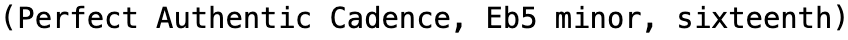
\includegraphics[width=0.45\textwidth]{images/perfauth_code}\\
\vspace{-2mm}
\noindent compiled and loaded into MuseScore notation software.
\vspace{-1mm}
\begin{figure}[h!]
\centering
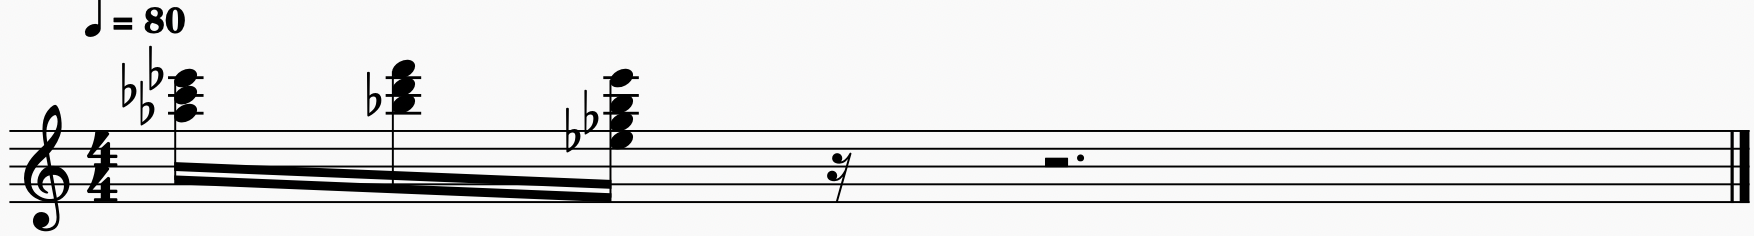
\includegraphics[width=0.45\textwidth]{images/perfauth}
  \caption{Perfect Authentic Cadence in E\musFlat\; minor \label{fig:perfauth}}
  \vspace{-3mm}
\end{figure}

Finally, harmonic sequences are specified by harmonic sequence type (ascending fifths, descending fifths, ascending 5-6, or descending 5-6), key, duration of each chord, and length of the sequence. Since MusAssist does not yet support multi-line composition, harmonic sequences are written like cadences in keyboard-style voice leading.

In music theory, harmonic sequences can be implemented in several ways depending on the desired inversion scheme. Though the upper-voice harmonization of a harmonic sequence need not follow the direction in the sequence’s name, MusAssist chooses a chord inversion and voice leading pattern such that each sequence does so. For instance, the Ascending Fifths sequence will ascend, and the Descending 5-6 sequence will descend. Each pattern also maximizes smooth voice leading. 

The chosen patterns for each MusAssist sequence are summarized in  \tabref{table:harmseq}.
All sequences are shown in major in this demonstration, but their minor counterparts are also supported. Each sequence consists of fourteen distinct chords before repeating in the subsequent octave. 
\vspace{-2mm}
\begin{table}[h!]

  \begin{center}
    \setlength{\maxcollen}{\widthof{vii$^{\text{o}{6 \atop 4}}$}}
    \resizebox{\columnwidth}{!}{
  \begin{tabular}{|c|@{}c@{}|}
  \hline
  Ascending Fifths  & \renewcommand{\arraystretch}{1.5}
                    \begin{tabular}{p{\maxcollen}p{\maxcollen}p{\maxcollen}p{\maxcollen}p{\maxcollen}} 
                        I$^{6 \atop 4}$ & V                & ii$^{6 \atop 4}$            & vi              & iii$^{6 \atop 4}$ \\ \hdashline
                        vii$^\text{o}$  & IV$^{6 \atop 4}$ & I                           & V$^{6 \atop 4}$ & ii                \\ \hdashline
                        vi$^{6 \atop 4}$ & iii             & vii$^{\text{o}{6 \atop 4}}$ & IV              
                    \end{tabular} \\ \hline 
  Descending Fifths & \renewcommand{\arraystretch}{1.5}
                    \begin{tabular}{p{\maxcollen}p{\maxcollen}p{\maxcollen}p{\maxcollen}p{\maxcollen}} 
                      I                & IV$^{6 \atop 4}$ & vii$^\text{o}$  & iii$^{6 \atop 4}$ & vi                          \\ \hdashline
                      ii$^{6 \atop 4}$ & V                & I$^{6 \atop 4}$ & IV                & vii$^{\text{o}{6 \atop 4}}$ \\ \hdashline
                      iii              & vi$^{6 \atop 4}$ & ii              & V$^{6 \atop 4}$
                    \end{tabular} \\ \hline
  Ascending 5-6     & \renewcommand{\arraystretch}{1.5}
                    \begin{tabular}{p{\maxcollen}p{\maxcollen}p{\maxcollen}p{\maxcollen}p{\maxcollen}} 
                      I     & vi$^6$ & ii              & vii$^{\text{o}6}$ & iii      \\ \hdashline
                      I$^6$ & IV     & ii$^6$          & V                 & iii$^6$  \\ \hdashline 
                      vi    & IV$^6$ & vii$^\text{o}$  & V$^6$           
                    \end{tabular} \\ \hline
  Descending 5-6    & \renewcommand{\arraystretch}{1.5}
                    \begin{tabular}{p{\maxcollen}p{\maxcollen}p{\maxcollen}p{\maxcollen}p{\maxcollen}} 
                      I$^{6 \atop 4}$ & V                & vi$^{6 \atop 4}$ & iii                         & IV$^{6 \atop 4}$ \\ \hdashline 
                      I               & ii$^{6 \atop 4}$ & vi               & vii$^{\text{o}{6 \atop 4}}$ & IV               \\ \hdashline 
                      V$^{6 \atop 4}$  & ii               & iii$^{6 \atop 4}$           & vii$^\text{o}$  
                    \end{tabular} \\ \hline
  \end{tabular}
  }
  
\caption{MusAssist Harmonic Sequences Summary}\label{table:harmseq}
\end{center}
\end{table}

\vspace{-8mm}
\subsection{Additional Features}
Beyond compositional elements, users can set the key signature at the beginning of any measure up to seven sharps or flats by specifying note name, accidental, and quality (sharp or flat). Users can also start a new measure or create a blank measure. Finally, users can assign MusAssist expressions to string labels and reuse them later in the program (the labels are syntactic sugar for the expressions). MusAssist comments are designated with \verb!//!.

The tempo for all MusAssist programs
is set to \musQuarter\;= 80bpm and cannot currently be changed.
This also apples to the time signature, which is set to \setmeter{4}{4}.

All compiled MusAssist programs adhere to standard notation conventions. Notes and rests are broken over barlines as well as over the strong beat (beat three) of the measure. They are divided greedily into valid rhythmic units (from sixteenth to whole note) ordered either least to greatest, or greatest to least in the case of spillage of a tied note over the barline into the following measure.
%-----------------------------------------------------------------------------------------------------------------------------------------------------
\section{Sample Program}\label{sec:sample_program}
The full breadth of MusAssist's syntax is demonstrated in \figref{fig:example_program_code}, and \figref{fig:example_program} presents the resulting compiled MusicXML code when opened in MuseScore. 

\begin{figure}[h!]
\centering
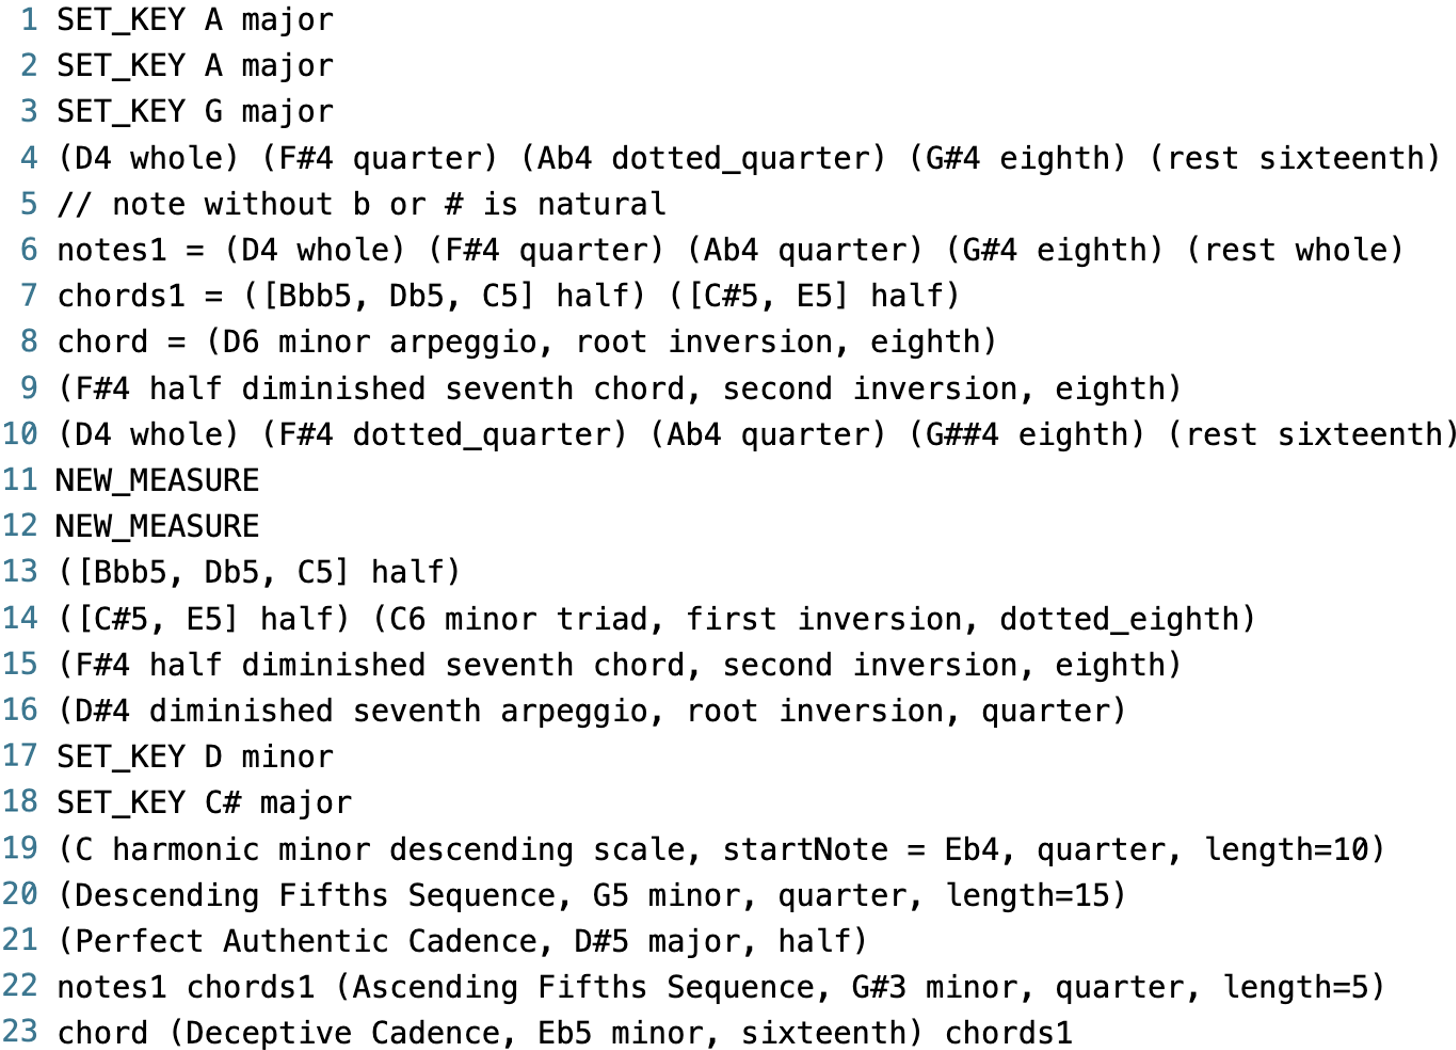
\includegraphics[width=0.5\textwidth]{images/example_program_code}
\vspace{-4mm}
\caption{MusAssist Syntax}\label{fig:example_program_code}
\end{figure}
\vspace{-6mm}
\begin{figure}[h!]
\centering
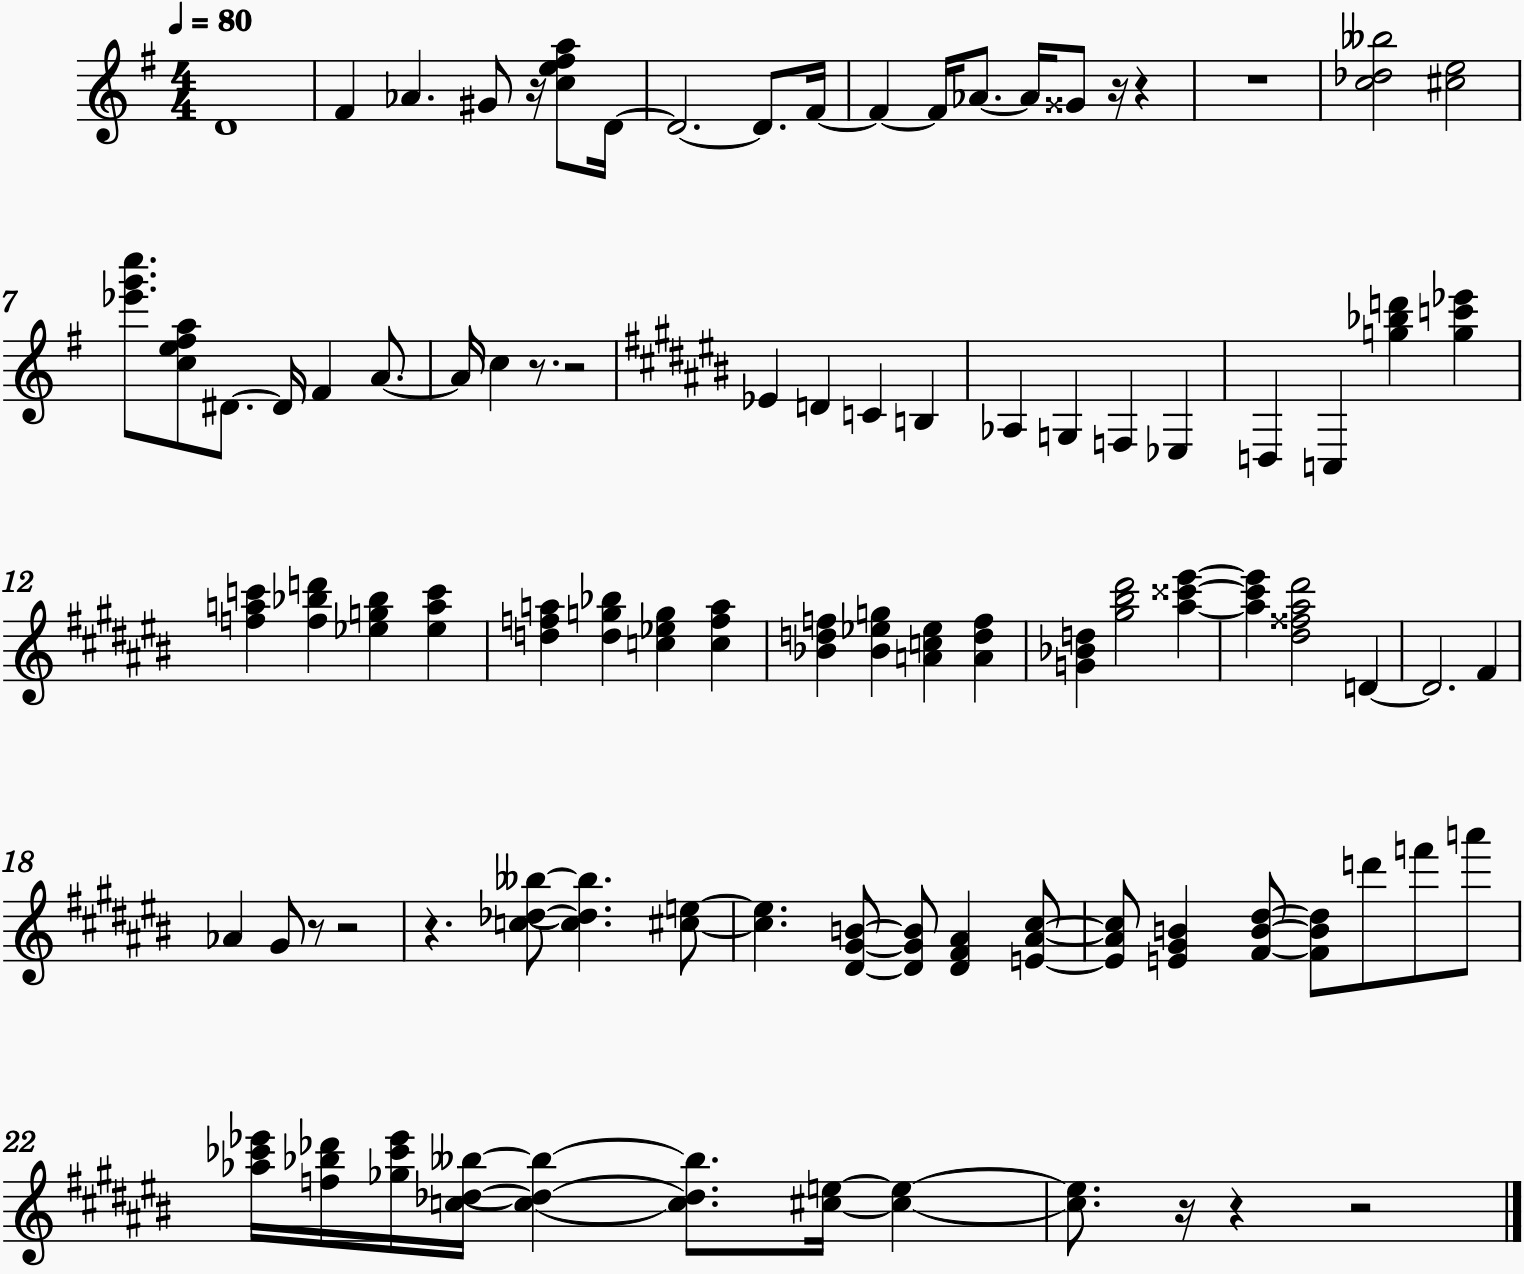
\includegraphics[width=0.5\textwidth]{images/example_program}
\caption{Compiled MusAssist Program in MuseScore}\label{fig:example_program}
\vspace{-3mm}
\end{figure}
  
Several features of MusAssist are clarified in Figures \ref{fig:example_program_code} and \ref{fig:example_program}:
\vspace{-2mm}
\begin{itemize}
\itemsep0em
\item The key signature can be changed consecutively as many times as desired, but only the last will take effect (as seen m. 1 and m. 12 of \figref{fig:example_program}). Changing the key signature triggers a new measure.
\item Note durations are automatically broken by the compiler both on the strong beat and on the barline (such as in mm. 2-4 of \figref{fig:example_program} ).
\item Labeled phrases are not notated until the label is referenced, rather than defined.
\item The difference between a customized chord and a chord template is exemplified on line 14 of \figref{fig:example_program_code}.
\end{itemize}
\vspace{-5mm}
%-----------------------------------------------------------------------------------------------------------------------------------------------------

\section{Compiler Structure}\label{sec:compiler_structure}

The MusAssist compiler is written in Haskell. Its high-level structure is as follows: 

\begin{enumerate}
\itemsep0em 
  \item MusAssist’s concrete syntax is parsed into abstract syntax, represented as Haskell algebraic data types (ADTs). Parser combinators were chosen for their flexibility and ease of customization. Parsec, an industrial strength parser library, is used, and Parsec’s helper module Token handles lexing. The parse preserves the abstraction level of all templates.

  \item All templates, now represented as ADTs, are expanded using the logic in Section 6 until the granularity reaches the note level. The result of this intermediate stage is abstract syntax whose abstraction level matches that of the target language, MusicXML.

  \item The low-level abstract syntax resulting from the fully expanded templates is translated to MusicXML. This step contains the temporal logic that subdivides notes and rests across barlines and strong beats.
  
\end{enumerate}

The resulting MusicXML file can then be opened in standard music notation software like MuseScore for viewing, further editing, and playback.

%-----------------------------------------------------------------------------------------------------------------------------------------------------

\section{Template Expansion Logic}\label{sec:template_expansions}
MusAssist’s distinguishing feature is its ability to automate the expansions of theoretical musical templates given user-supplied specifications at a higher level of abstraction. The logic underlying the expansions is summarized below. 

\subsection{Backbone Logic}
\subsubsection{Generating Notes in a Diatonic Scale}
\label{sec:note_generate}
Most MusAssist templates are built upon the diatonic scale. To automate the expansions of these templates, we must first be able to generate a note in a desired diatonic scale given a positive interval within one octave of the specified tonic. Recall that a MusAssist note is defined by note name, octave, and accidental. Given the target interval $n$, to determine the note name we begin at the tonic and travel $n$ steps up MusAssist’s custom Haskell ADT for note names, a circular Enum instance ordered as the C major scale is. 

The desired octave is either the same as that of the tonic, or one greater if the desired note name (disregarding accidental) comes before the tonic note name in the C major scale. For instance, as seen in \figref{note_octaves}, the red note names D, E, and F come before G in the C major scale, and the octave number of each is one higher than the tonic in a G major scale.

\vspace{-2mm}
\begin{figure}[h!]
\centering
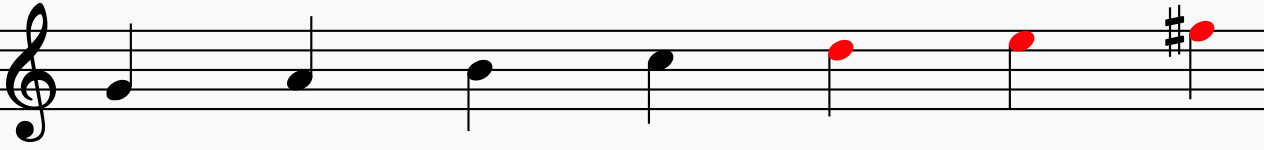
\includegraphics[width=0.3\textwidth]{images/note_octave_logic}
\caption{\centering Octave Analysis of G Major Scale}
\label{note_octaves}
\vspace{-3mm}
\end{figure}

To determine the desired accidental, first realize that in any key, a perfect interval will generally have the same accidental as the tonic, with two exceptions: the perfect fifth above B is F\musSharp, and the perfect fourth above F is B\musFlat. To work out the logic behind the accidental of a desired imperfect interval, consider \figref{maj_seconds}. Here, we consider all single-accidental key signature names (even invalid ones that contain double sharps or flats) in order to establish the pattern. Key signature names are grouped under the accidental of the note that is the desired interval from the tonic. For instance, in the key of A\musFlat\;, the major second interval from the tonic is B\musFlat. The accidental of B\musFlat\; is \musFlat, so A\musFlat\; falls under the \musFlat\; column in \figref{maj_seconds}.
\vspace{-2mm}
\begin{figure}[h!]
\centering
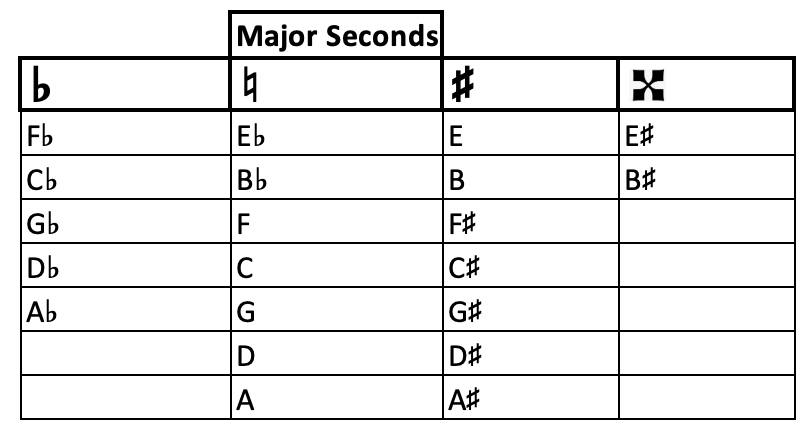
\includegraphics[width=0.3\textwidth]{images/maj_seconds}
\caption{Accidental of Major Second from Tonic per Key}
\label{maj_seconds}
\vspace{-2mm}
\end{figure}

From \figref{maj_seconds} we see that given any key, the major second above the tonic has the same accidental as the tonic, except for any key with E or B in its name. In these keys, the accidental is ``lifted"   (i.e. \musFlat $\rightarrow$ \musNatural, \musNatural $\rightarrow$ \musSharp, and \musSharp $\rightarrow$ \musDoubleSharp).

A similar pattern emerges for minor thirds, major sixths, and minor sevenths from the tonic. Using the result of this analysis, we can determine the accidentals of the inverse qualities (i.e. major versus minor) of the imperfect intervals by either lowering the computed accidental when going from major to minor, or lifting it otherwise. Augmented and diminished intervals from the tonic are not considered since they do not appear in diatonic scales.

\subsubsection{Generating Chord Templates in a Diatonic Scale}
\label{sec:chord_generate}
Generating chord templates in a diatonic scale becomes relevant for the expansions of the highest-level MusAssist templates – namely, cadences and harmonic sequences – that are defined in music theory by lists of chord templates rather than notes. 

The goal here is to automate the generation of chord templates for triads in a diatonic scale given a specified tonic tone and quality for the scale (major or minor), inversion, and positive interval within one octave of the tonic for the chordal root. If we need to generate a chord template for a seventh chord, we simply generate the base triad and add the fourth note afterwards. 

In order to complete the triad template definition from the supplied information, we simply need to determine the desired chord quality. Music theory dictates that the major diatonic scale contains the triads  I-ii-iii-IV-V-vi-vii$^\text{o}$, and the minor diatonic scale contains the triads i-ii$^\text{o}$-III-iv-v-VI-VII. Using this, we can thus compute the triad quality given the tonic quality and the supplied interval between tonic and desired chordal root.

\subsection{Template Expansions}
\subsubsection{Scales}
The expansion of all major and natural/harmonic/melodic minor scales is derived from the logic in Section \ref{sec:note_generate}. The scale is generated in relation to its tonic, rather than the specified starting note. The tonic octave is always set so that the tonic falls below the start note. This ensures that the initial interval between tonic and start note is positive, with the interval then increasing for ascending scales and decreasing for descending scales until the desired scale length is reached. If the tonic is reached in the scale generation, we reset the tonic to be one octave higher or lower (depending on the scale direction) so that the interval between the next note in the scale and the current tonic is always positive and within a single octave. Finally, consider that all minor scales are treated as natural when generating their notes. If needed, the notes are modified afterwards in order to appropriately raise the sixth and/or seventh scale degree(s) for harmonic and melodic minor scales. For the non-diatonic scales (chromatic and whole tone), C is set as the “tonic” for the purposes of determining the octave. As with diatonic scales, the tonic octave is shifted appropriately if it is passed during the scale generation.

As seen in \figref{chromatic}, for 10 of the 12 tones, chromatic scales “double” the note name, with the directional accidental (sharp for ascending, flat for descending) falling on the second occurrence. The two exceptions marked in red in \figref{chromatic} are E and B in the ascending version and C and F in the descending version.
\vspace{-2mm}
\begin{figure}[h!]
\centering
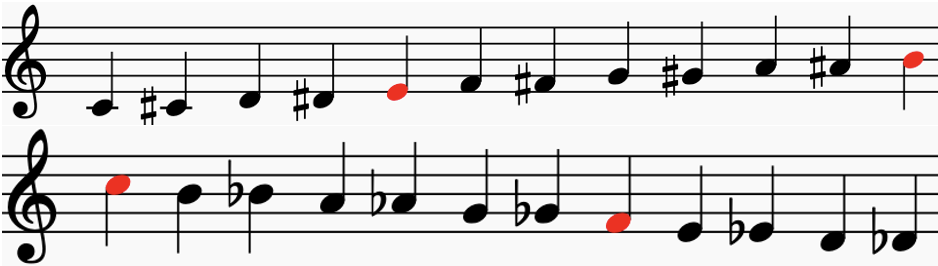
\includegraphics[width=0.4\textwidth]{images/chromatic}
\caption{Chromatic Scales}
\label{chromatic}
\vspace{-3mm}
\end{figure}

If we are on a single note, we simply move up the scale. Otherwise, we repeat it and insert an accidental on the second occurrence.

Whole tone scales are constructed with a similar model. As seen in \figref{chromatic}, the ascending whole tone scale is missing the note B, while the descending is missing C.

\vspace{-2mm}
\begin{figure}[h!]
\centering
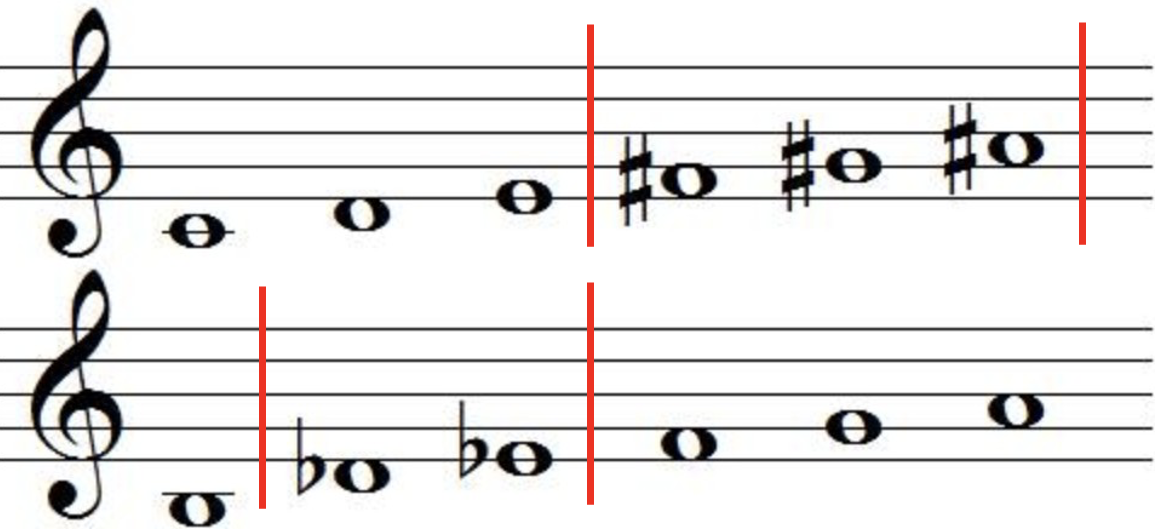
\includegraphics[width=0.25\textwidth]{images/whole_tone}
\caption{Whole Tone Scales}
\label{whole_tone}
\vspace{-3mm}
\end{figure}

To determine the next note name, we thus simply traverse up or down the C major scale, excluding the appropriate tone. To determine the next accidental, we appropriately lift or lower the current accidental if we reach one of the red boundaries in \figref{whole_tone}, otherwise leaving it unchanged.

\subsubsection{Chords and Arpeggios}
\label{sec:chord_expansion}
Each note in a chord or arpeggio is generated with the logic from Section \ref{sec:note_generate} based on its interval from the tonic (i.e. the chordal root). Chordal thirds, fifths, and sevenths have respective intervals of 2, 4, and 6 from the tonic.

The imperfect chordal intervals are initially set to major for major, dominant, and augmented chords, and to minor for minor, half diminished, and fully diminished chords. Thus, after the note is generated, for augmented chords the chordal fifth accidental must be lifted, and the seventh must be lowered. For dominant seventh chords, the seventh must be lowered. Finally, for diminished chords, the fifth and seventh must be lowered, and for half diminished seventh chords, the fifth alone must be lowered.

To handle inversions, recall that the chord (whether triad or seventh) starts out in root position. Let $n$ be the desired inversion value (0 for root, 1 for first inversion, 2 for second, and 3 or third). By incrementing the octaves of the first $n$ tones of the chord in root position, we obtain the correct inversion.

If the chord is specified as an arpeggio, we simply return a series of individual notes, rather than a simultaneous cluster.

\subsubsection{Cadences}
A cadence must undergo two levels of expansion: an intermediate step from the cadence to the list of chord templates it defines, and a final step from chord templates to notes.

Recall that the chords in each cadence are defined in Section \ref{table:cadences}, which reveal the interval of each chordal root from the tonic. Using this, for each chord in the cadence, we first employ the logic from Section \ref{sec:note_generate} to generate the root note of each chord. Then, we use the logic in Section \ref{sec:chord_generate} to generate a template for each chord, which undergoes a second expansion in Section \ref{sec:chord_generate}.

The scale quality given in Section \ref{sec:chord_generate} to generate the chord template is generally that of the cadence. However, there are exceptions. All V chord templates are generated within a major scale, no matter the cadence quality, since cadences always have major V chords. Similarly, we want the seventh triad in the imperfect authentic cadence to be diminished – i.e. built on the major seventh scale degree – no matter the local key quality, since we raise the leading tone in minor keys when moving towards the tonic. Thus, this chord template must also be generated within a major scale in Section \ref{sec:chord_generate}.

The tonic octave supplied for the chord template generation in Section \ref{sec:chord_generate} is also usually that of the cadence. However, in order for the cadences to follow smooth voice leading, the tonic octave must be lowered once in relation to the specified cadence octave when generating second inversion triads, which appear in all cadences except perfect authentic. This is demonstrated in the B major deceptive cadence in \figref{fig:cadence_octaves}. After converting to root position for clarity, note that the chordal root in the cadence octave is in blue and the roots an octave below (i.e. those of the second inversion triads) are in red.

\vspace{-2mm}
\begin{figure}[h!]
\centering
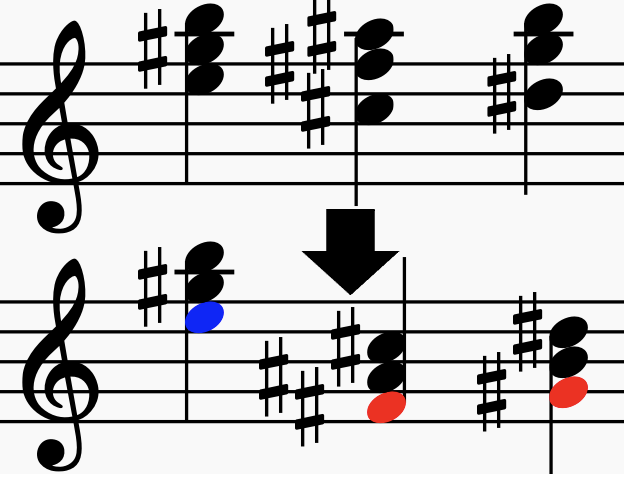
\includegraphics[width=0.18\textwidth]{images/cadence_octaves}
  \caption{Deceptive Cadence Octave Analysis}\label{fig:cadence_octaves}
\end{figure}
\vspace{-4mm}

\subsubsection{Harmonic Sequences}
Like cadences, harmonic sequences are initially expanded to the chord templates they comprise, which then undergo a second expansion to notes. Recall from \figref{table:harmseq} that each sequence consists of 14 chords, after which it cycles an octave above or below, depending on the direction of the sequence.

In order to generate chord templates for a sequence, we need to determine:

\vspace{-1mm}
\begin{enumerate}
\itemsep0em 
\item The interval between each pair of chordal roots, which dictates how to proceed from one chord to the next in the sequence
\item The inversion of each chord
\item The octave number of each chord (given by the chordal root octave) relative to the tonic
\end{enumerate}


To determine (1) and (2), consider the analysis in \figref{fig:desc_56_intervals}, which determines the interval pattern for the chordal roots of the descending 5-6 sequence (as defined previously in \figref{table:harmseq}), given the zero-based index of each chord in the sequence.

\begin{figure}[h!]
\centering
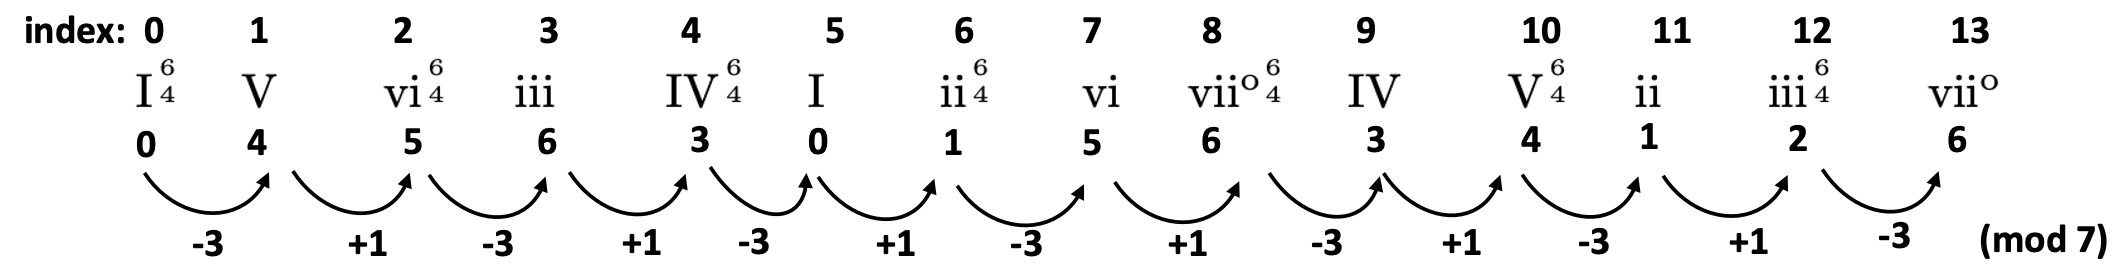
\includegraphics[width=0.5\textwidth]{images/desc_56_intervals}
  \caption{Descending 5-6 Interval Analysis}\label{fig:desc_56_intervals}
\end{figure}
\vspace{-3mm}

The top row is the chord index, the second row is the chord progression from \tabref{table:harmseq}, the third row is the interval between each chordal root and the tonic, and the bottom row is the interval between each chordal root and the previous (modulo 7). A clear pattern for inversions (in the second row) and interval changes (in the fourth row) emerges based on the parity of the index. Identical analyses are applied to the remaining sequences to formalize their interval and inversion patterns.

Finally, we need to determine (3), the octave number of each chordal root relative to the tonic, or the root of the first chord in the sequence. Consider \figref{fig:desc56-example}, which presents an octave analysis for the descending 5-6 sequence.

\vspace{-2mm}
\begin{figure}[h!]
\centering
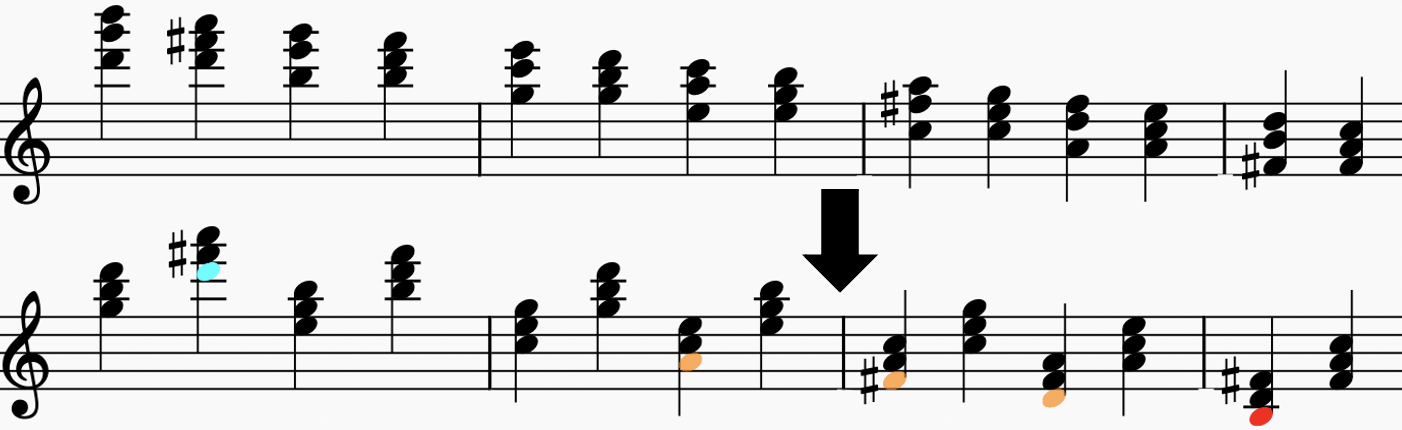
\includegraphics[width=0.45\textwidth]{images/desc56-example}
  \caption{Descending 5-6 Octave Analysis}
  \label{fig:desc56-example}
\end{figure}
\vspace{-3mm}

In \figref{fig:desc56-example}, all chords are converted to root position in order to visualize the octave numbers of their roots in relation to the tonic. The chordal roots in blue are an octave number above the tonic, the roots in yellow are an octave below, and the root in red is two octaves below. This same analysis is applied to determine the octave numbers of the chords in the remaining sequences.

Importantly, the interval analysis in \figref{fig:desc_56_intervals} holds for any representation of a harmonic sequence, as this is what defines the musical theoretical structure. However, the inversion and octave analyses in Figures \ref{fig:desc_56_intervals} and \ref{fig:desc56-example} hold only for MusAssist’s chosen representation of the sequences in \tabref{table:harmseq}, as a different inversion scheme would alter their outcomes.

%-----------------------------------------------------------------------------------------------------------------------------------------------------

\section{Conclusion}
This paper presents MusAssist, an external, declarative DSL for music notation that closes the abstraction gap between music theory and written composition. Users can uniquely write specifications in MusAssist’s simple and high-level syntax for scales, chords, arpeggios, cadences, and harmonic sequences at the precisely levels of abstraction of the theoretical musical structures they describe. Fundamental musical elements such as notes, rests, custom note collections, new measures, and key signatures are also supported, along with the ability to reuse labeled expressions and indicate comments. MusAssist programs are translated by its Haskell-based compiler to MusicXML, enabling the composition to be loaded into notation software for further manual editing.


Optimally, in the future, MusAssist would support templates for additional non-diatonic structures like octatonic and pentatonic scales, as well as all flavors of suspended, ninth, eleventh, and thirteen chords (often seen in jazz). Templates for key modulations are also planned, which would provide specifications that generate a sequence of chords modulating from a start key to a target key. Furthermore, future versions of MusAssist will allow for increased customizability of existing templates that are not currently fully expressive. The present MusAssist template expansions for cadences and harmonic sequences are limited to the representation schemes outlined in Tables \ref{table:cadences} and \ref{table:harmseq}. In order for MusAssist to fully close the abstraction gap between theoretical musical structures and their low-level notational forms, all functional harmonic variations should be supported. Additionally, support for two-clef, multi-staff composition would improve the implementation of cadences and harmonic sequences by including the essential baseline. Finally, user studies of MusAssist would give insight into potential improvements for language design.

\begin{acknowledgments}
I am very grateful to Professor Ben Wiedermann of Harvey Mudd College for his invaluable mentorship throughout this project.
\end{acknowledgments} 

%%%%%%%%%%%%%%%%%%%%%%%%%%%%%%%%%%%%%%%%%%%%%%%%%%%%%%%%%%%%%%%%%%%%%%%%%%%%%
%bibliography here
\bibliography{icmc2021template}

\end{document}
